%\documentclass{scrartcl}
\documentclass[11pt,twocolumn]{article}
\usepackage{a4wide}
\usepackage[a4paper, left=1.3cm, right=1.3cm, bottom=2cm]{geometry}

\usepackage{amsmath,amsfonts,amssymb}
\usepackage{xfrac}
\usepackage{graphicx}
%\usepackage{tikz}
%\usetikzlibrary{calc}
\usepackage{fancybox}
\usepackage{xcolor}


\usepackage{tikz}
\usetikzlibrary{scopes}



\newcommand{\be}{\begin{equation}}
\newcommand{\ee}{\end{equation}}

\newcommand{\bel}[1]{\begin{equation}\label{#1}}
\newcommand{\eel}{\end{equation}}

\newcommand{\bea}{\begin{eqnarray*}}
\newcommand{\eea}{\end{eqnarray*}}

\newcommand{\eq}  [1] {\be #1 \ee}
\newcommand{\eql} [2] {\bel \label{#1} #2 \eel}

\newcommand{\w}{\omega}
\newcommand{\ka}{\varkappa}

\newcommand{\Dr}{\Delta_r}
\newcommand{\Sr}{\Sigma_r}
\newcommand{\Dp}{\Delta_\phi}
\newcommand{\Sp}{\Sigma_\phi}

\hyphenation{wave-let}


\newcommand {\WT} {$\mathcal{W}_{\!\psi}x$ }
\newcommand {\z}   {z^{-1}}

\newcommand{\rbox}[1]{\colorbox{red!10}{$#1$}}
\newcommand{\gbox}[1]{\colorbox{green!10}{$#1$}}
\newcommand{\bbox}[1]{\colorbox{blue!10}{$#1$}}

\newcommand{\um}{\scalebox{0.65}[1.0]{\( - \)}}  % unary minus

\newcommand{\leftshift}{\triangleleft}
\newcommand{\rightshift}{\triangleright}
%\newcommand{\leftshift}{\vartriangleleft}
%\newcommand{\rightshift}{\vartriangleright}
%\newcommand{\leftshift}{\blacktriangleleft}
%\newcommand{\rightshift}{\blacktriangleright}




\setlength{\columnseprule}{0.1pt}
\setlength{\columnsep}{1cm}


\graphicspath{ {figures/} }

\newcommand{\Fig}[4]{
\begin{figure}[htbp]
  \centering
  \includegraphics[width=#2]{#1}
  \caption{#4}
  \label{#3}
\end{figure}
}







\begin{document}

\title{Fast Gabor notes}
\author{Andr\'e Bergner}
\maketitle

    \section{Introduction}

motivation:

- continuous version: motivated by biology: cochlea: driven membrane

- discrete version: motivated technically/dsp: coupled filter-bank -> high-dimensional state space filter, where every sub-space is one desired filter output

  \subsection{Open Problems}

- yet no closed solution for full discrete version

- no analytic approach for non equally spaced frequencies, especially for log-scaled frequency distribution

- no better understanding of borders, if introduced. Currently lead to instabilities if to 'unsmooth'

  - stability: double is good, float is bad\\
- is implicit version more stable?

  - faster implicit version?\\
- serial filtering has less adds then parallel version\\
- skip infinite tail, use just tails from neighbor mirror unit circle half\\
- thus this would be three filters fwd, bwd w/ nieghbor, fwd neighbor




% --------------------------------------------------------------------------------------------------
\section{Continuous Version}
% --------------------------------------------------------------------------------------------------



% --------------------------------------------------------------------------------------------------
\subsection{Diffusion}


\be \label{pde}
   \rbox{\partial_t u = (\gamma + i x + \varkappa \partial_x^2 ) u  +  f(t),}
\ee
where $u(x,t)$ is the deviation of the membrane from it point of rest, $\gamma$ is the damping coefficient,
$\omega x$ is the inhomogeneous frequency term and $\varkappa$ the membrane's coupling strength (TODO correct term).

The solution of the unforced system ($f \equiv 0$) can be found analytically. We use the ansatz
\be \label{ansatz1}
   u(x,t) = e^{at + bt^2 + ct^3} e^{ixt}
\ee
Inserting (\ref{ansatz1}) into (\ref{pde}) one obtains
$$
   a  +  2 b t  +  3 c t^2  +  ix \; = \; \gamma + i x - \varkappa t^2,
$$
and after collecting all terms the coefficients can be determined to be $a=\gamma$, $b=0$, and $\varkappa = -3c$
which leaves us with the final solution
\be \label{pde-solution}
   \gbox{u(x,t) = e^{\gamma t - \varkappa t^3/3} e^{ixt}}
\ee

Conclusion: $\gamma$ has to be positive (unstable) for gaussian response shape,
any positive $\varkappa$ immedietely stabilizes the system




% --------------------------------------------------------------------------------------------------
\subsection{Advection --- true gaussian}


\be \label{pde2}
    \rbox{\partial_t u = (\gamma + i x + \varkappa \partial_x ) u  +  f(t),}
\ee
Substituting the ansatz for the homogenous solution ($f \equiv 0$) in (\ref{pde2})
\be \label{pde2ansatz}
   u(t) = \alpha(t) e^{ixt}
\ee
and its derivatives
\bea
   \partial_t u  &=&  ( \dot{\alpha} + ix\alpha ) e^{ixt} = ( \dot{\alpha} + ix\alpha ) \frac{u}{\alpha}\\
   \partial_x u  &=&  it\alpha e^{ixt} = itu
\eea
we get
\bea
   ( \dot{\alpha} + ix\alpha ) \frac{u}{\alpha}  &=&  (\gamma + i x) u + \varkappa itu\\
     \dot{\alpha} + ix\alpha  &=&  (\gamma + i x + \varkappa it ) \alpha\\
     \dot{\alpha}  &=&  (\gamma + \varkappa it) \alpha\\
\eea
which can be solved by separation of variables
\be
   \int\! \frac{d\alpha}{\alpha} \ =\  \int\!\! dt \; (\gamma + \varkappa it).
\ee
The solution is
\be
   \log \alpha \ = \ c + \gamma t + \frac{i\varkappa}{2} t^2.
\ee
The integration constant $c$ would be found from the initial conditions and can be factored out and will be set to 0. From the solution it's clear that in order to obtain a gaussian envelope $\varkappa$ must be pure imaginary. Thus by replacing $\varkappa \rightarrow -i\varkappa$ we get the differential equation
\be \label{pde2a}
   \partial_t u = (\gamma + i x - i\varkappa \partial_x ) u  +  f(t),
\ee
with the homogenous solution
\be \label{pde2a_solution}
    \gbox{u(x,t) \ = \ e^{\gamma t - \varkappa t^2 / 2} e^{ixt}}
\ee



% --------------------------------------------------------------------------------------------------
\subsection{scale invariant advection -- Wavelet filterbank}

We modify Eq. \ref{pde2} to scale the frequencies exponentially ($x \rightarrow e^x$) and also make
the damping scale accordingly ($\gamma \rightarrow \partial_x e^x = e^x$).
\be \label{wlet_adv_pde}
    \rbox{\partial_t u = e^x (\gamma + i + \varkappa\partial_x) u  +  f(t),}
\ee

The ansatz condition is that the solution must be scale invariant, that is
\be \label{wlet_adv_ansatz}
    u(x,t) = \phi(e^xt).
\ee
Substituting the ansatz and its derivatives
\bea
   \partial_t u  &=&  \phi^\prime e^x \\
   \partial_x u  &=&  \phi^\prime t e^x
\eea
in Eq. \ref{wlet_adv_pde} we get
\be
   \phi^\prime e^x  =  e^x(\gamma + i)\phi + \varkappa\phi^\prime t e^{2x}.
\ee
Substituting $\tau = e^xt$ yields the ordinary differential equation
\bea
   \phi^\prime  &=&  (\gamma + i) \phi + \varkappa\tau\phi^\prime \\
   \phi^\prime (1 - \varkappa\tau)  &=&  (\gamma + i) \phi
\eea
which can be solved by separation of variables
\be
   \int\! \frac{d\phi}{\phi} \ =\  \int\!\! d\tau \; \frac{\gamma + i}{1 - \varkappa\tau}.
\ee
The solution is
\be
   \ln \phi \ = \ c - (\gamma + i) \frac{1 - \varkappa\tau}{\varkappa}
\ee
Substituting back $t$ and letting $c=0$ we have the homogenous solution for (\ref{wlet_adv_pde})
\be \label{wlet_adv_solution}
    \gbox{ u(x,t) \ = \ \exp\!\big(-\!\frac{\gamma+i}{\varkappa} \; ln(1-\varkappa e^x t)\big) }
\ee








% --------------------------------------------------------------------------------------------------
\subsection{Spatially discretized -- Advection}


Nabla is discretized by 2nd order finite difference scheme:
\be \label{pdiffe}
    \rbox{\partial_t u_n = (\gamma + i n) u_n - i \ka ( u_{n+1} - u_{n-1} )  +  f(t),}
\ee
(TODO: there should be an $\w$ factor ?)

Using the usual ansatz
\be
   u(t) = \alpha(t) e^{int}
\ee
with
\bea
    \partial_t u_n       &=&  ( \dot{\alpha} + in\alpha ) e^{int} = ( \dot{\alpha} + in\alpha ) \frac{u}{\alpha}\\
              u_{n\pm 1} &=&  e^{\pm it} u_n
\eea
in Eq. (\ref{pdiffe}) yields
\bea
   ( \dot{\alpha} + in\alpha ) \frac{u_n}{\alpha}  &=&  (\gamma + i n) u_n - i \ka (e^{+it}-e^{-it}) u_n \\
     \dot{\alpha} + in\alpha  &=&  \big((\gamma + i n) + 2 \ka \sin t \big) \alpha \\
                \dot{\alpha}  &=&  \big( \gamma + 2 \ka \sin t \big) \alpha,
\eea
an ordinary differential equation for the amplitude which can be solved by separation of variables
\be
   \int\! \frac{d\alpha}{\alpha} \ =\  \int\!\! dt \; ( \gamma + 2\ka\sin t ).
\ee
The solution is
\be
   \log \alpha \ = \ c + \gamma t - 2\ka \cos t
\ee
Thus we get the homogenous solution for Eq. (\ref{pdiffe}) ($c=0$)
\be
   \gbox{u(x,t) \ = \ e^{\gamma t - 2\ka \cos t} e^{int}}
\ee





% --------------------------------------------------------------------------------------------------
\subsection{Spatially discretized -- Diffusion}


This version has the spatial laplacian term discretized by finite difference scheme (classical discrete laplacian):
\be \label{pdiffe}
    \rbox{\partial_t u_n = (\gamma + i n) u_n + \ka ( u_{n-1} - 2u_n + u_{n+1} )  +  f(t),}
\ee
(TODO: there should be an $\w$ factor ?)

Using the usual ansatz
\be
   u(t) = \alpha(t) e^{int}
\ee
with
\bea
    \partial_t u_n       &=&  ( \dot{\alpha} + in\alpha ) e^{int} = ( \dot{\alpha} + in\alpha ) \frac{u}{\alpha}\\
              u_{n\pm 1} &=&  e^{\pm it} u_n
\eea
in Eq. (\ref{pdiffe}) yields
\bea
   ( \dot{\alpha} + in\alpha ) \frac{u_n}{\alpha}  &=&  (\gamma + i n) u_n + \ka (e^{+it}+e^{-it}-2) u_n \\
     \dot{\alpha} + in\alpha  &=&  \big((\gamma + i n) + \ka 2(\cos t-1) \big) \alpha \\
                \dot{\alpha}  &=&  \big( \gamma + 2\ka(\cos t-1) \big) \alpha,
\eea
an ordinary differential equation for the amplitude which can be solved by separation of variables
\be
   \int\! \frac{d\alpha}{\alpha} \ =\  \int\!\! dt \; \big( \gamma + 2\ka(\cos t-1) \big).
\ee
The solution is
\be
   \log \alpha \ = \ c + (\gamma-2\ka) t + 2\ka \sin t
\ee
Thus we get the homogenous solution for Eq. (\ref{pdiffe}) ($c=0$)
\be
   \gbox{u(x,t) \ = \ e^{(\gamma-2\ka) t + 2\ka \sin t} e^{int}}
\ee

Conclusion: The adjecency version is better suited as the stability is merely controlled by $\gamma$
whereas $\varkappa$ controls ...





  \subsection{discrete time, continuous space}

\be
    \rbox{u^{t+1} = re^{ix} ( u^t  +  \ka \partial_x^2 u^t )}
\ee
Ansatz:
\be
   u^t = \alpha^t e^{ixt}
\ee
with
\bea
    u^{t+1}           &=&  \alpha_{t+1} e^{ix} e^{ixt} \ = \ e^{ix} \frac{\alpha_{t+1}}{\alpha_t} u^t \\
    \partial_x^2 u^t  &=&  -t^2 \alpha_t e^{ixt} \ = \ -t^2 u^t
\eea
inserting:
\bea
     e^{ix} \frac{\alpha_{t+1}}{\alpha_t} u^t  &=&  re^{ix} ( 1 - t^2\ka ) u^t \\
     \alpha_{t+1}  &=&  \alpha_t r ( 1 - \ka t^2 )
\eea
This difference equation for $\alpha$ diverges for all non-zero values of $\ka$.





  \subsection{Full discrete version}

The spatially discretized Eq. (\ref{pdiffe})
$$
    \rbox{\partial_t u_n = \big[ (\gamma + i \w n) + \ka ( \mathbb{S}_{-1} + \mathbb{S}_{+1} )\big] u_n}
$$
(here in it's adjacency formulation) has the general solution
\be \label{discrete_projection}
    \mathbf{u}(t) = e^{t \big[ (\gamma + i \w n) + \ka ( \mathbb{S}_{-1} + \mathbb{S}_{+1} )\big]} \mathbf{u}(0)
\ee
which can be rewritten as a difference equation by iterating the solution step-wise
$$
    \mathbf{u}(t+1) = e^{\gamma + i \w n} e^{\ka ( \mathbb{S}_{-1} + \mathbb{S}_{+1} )} \mathbf{u}(t)
$$
The second exponential can be expanded which yields
$$
    \mathbf{u}(t+1) = e^{\gamma + i \w n} \big( 1 + \ka ( \mathbb{S}_{-1} + \mathbb{S}_{+1} ) + \dots \big) \mathbf{u}(t)
$$
We cut off after the second term of the expansion in order to maintain the same algebraic complexity and the same coupling depth as the original differential equation. Introducing a shorter notation for time and space indices and applying the shift operator to the state $u$ yields



\be \label{diffeq}
   u_n^{t+1} = re^{i\w n} \big( u_n^t  +  \varkappa ( u_{n-1}^t + u_{n+1}^t ) \big)  +  f^t.
\ee
Inserting the ansatz
\be \label{diffeq_ansatz}
   u_n^t = \alpha^t e^{i\w nt}
\ee
in (\ref{diffeq}) ($f \equiv 0$) with corresponding shifted versions
\bea
    u_n^{t+1}    &=&  \alpha_{t+1} e^{i\w n} e^{i\w nt} \\
                 &=&  e^{i\w n} \frac{\alpha_{t+1}}{\alpha_t} u_n^t \\
    u_{n\pm 1}^t &=&  e^{\pm i\w t} u_n^t
\eea
yields
\bea
    e^{i\w n} \frac{\alpha_{t+1}}{\alpha_t} u_n^t  &=&
        re^{i\w n} \big( u_n^t +  \varkappa ( e^{-i\w t} + e^{+i\w t} ) u_n^t \big) \\
    \frac{\alpha_{t+1}}{\alpha_t}  &=&  r ( 1 + \varkappa ( e^{-i\w t} + e^{+i\w t} )) \\
    \alpha_{t+1}  &=&  r ( 1 + 2 \varkappa \cos(\w t) ) \alpha_t
\eea
Thus, the solution for $\alpha_t$ will be
\bea
    \alpha_t &=& \alpha_0 \prod_{\tau=1}^t r ( 1 + 2 \varkappa \cos(\w \tau) ) \\
    \alpha_t &=& \alpha_0 r^t \prod_{\tau=1}^t ( 1 + 2 \varkappa \cos(\w \tau) ) \\
\eea

Side notes: By introducing $a_t = \log \alpha_t$ the above equation can be read
$$
   a_{t+1} = a_{t} + \log r + \log( 1 + 2\varkappa \cos \w t )
$$

\mbox{ }

\mbox{ }

Open problem: find solution of $\prod(1+2\dots)$ or $\sum\log(1+2\dots)$, respectively.
\be\begin{split}
    &\!\!\!\prod_t (1 + 2\ka\cos t) \\
    &\ \ \ = (1 + 2\ka\cos 0)(1 + 2\ka\cos 1)(1 + 2\ka\cos 2)\dots\\
    &\ \ \ = 1 + 2\ka ( \cos 0 + \cos 1 + \cos 2 + \dots) + \dots
\end{split}\ee



\subsubsection{Scaling}

Eq. (\ref{discrete_projection}) is of the form
$$
  \mathbf{u}(t) = e^{t \mathbb{P}} \mathbf{u}(0)
$$
with $\mathbb{P} = (\gamma + i \w n) + \ka ( \leftshift + \rightshift )$ being the continuous time operator,
where $\leftshift$ and $\rightshift$ denote the left-shift ($\mathbb{S}_{-1}$) and right-shift ($\mathbb{S}_{+1}$)
operators, respectively.
By choosing different time steps than unity, say $\tau$, the discrete time version can be scaled arbitrary:
$$
  \mathbf{u}(t+\tau) = e^{\tau \mathbb{P}} \mathbf{u}(t)
$$
Thus, the general version of Eq. (\ref{diffeq}) is
\bea
  \mathbf{u}(t+1) &=& e^{\tau(\gamma + i \w n)} e^{\tau\ka ( \leftshift + \rightshift )} \mathbf{u}(t)\\
                   &=& e^{\tau(\gamma + i \w n)} \big(1 + \tau\ka ( \leftshift + \rightshift ) + \dots \big) \mathbf{u}(t)\\
             &\approx& e^{\tau(\gamma + i \w n)} \big(1 + \tau\ka ( \leftshift + \rightshift )\big) \mathbf{u}(t)
\eea

So we arrive at the scaleable discrete time, discrete space filter bank:
\be \label{dsdt_rescaled}
    \mathbf{u}_{t+1} = e^{\tau(\gamma + i \w n)} (1 + \tau\ka ( \leftshift + \rightshift )) \mathbf{u}_t
\ee







\subsubsection{Transfer function}

The partial difference equation (\ref{diffeq}) in matrix form is written
$$
    \mathbf{u}_{t+1} = \mathbf{A}\big( \mathbf{1} + \ka \mathbf{K} \big) \mathbf{u}_t + \mathbf{B}f_t
$$
where $ \mathbf{A} = diag\{a_n\!\!=\!e^{\gamma + i \w n}\}$.
Applying the z-tranform with yields
$$
    z\mathbf{U}(z) = \mathbf{A}\big( \mathbf{1} + \ka \mathbf{K} \big) \mathbf{U}(z) + \mathbf{B}F(z)
$$
Rearranging for the definition of the transfer function $\mathbf{H}(z) = \mathbf{U}(z)/F(z)$
$$
    \big[ z \mathbf{1} - \mathbf{A}\big( \mathbf{1} + \ka \mathbf{K} \big) \big] \mathbf{H}(z) = \mathbf{B}
$$
and thus
$$
    \mathbf{H}(z) = \big[ z \mathbf{1} - \mathbf{A}\big( \mathbf{1} + \ka \mathbf{K} \big) \big]^{-1} \mathbf{B}
$$

%\be \label{eq:discrete_laplacian}
%\begin{pmatrix}
%       1 & \um1 &       & &           \\
%    \um1 &    2 &  \um1 & &           \\
%         &      & \dots & &           \\
%       &      &  \um1 &    2 & \um1 \\
%         &      &       & \um1 &  1
%    \end{pmatrix}
%\ee

\be
\begin{pmatrix}
      1 & \ka &        &      & \ka  \\
    \ka &    1 &  \ka  &      &      \\
        &      & \dots &      &      \\
       &      &  \ka  &    1 & \ka  \\
    \ka &      &       & \ka  &   1
    \end{pmatrix}
\ee






%     -----------------------------------------------------------------------------------------
%    DISCRETIZATION
%     -----------------------------------------------------------------------------------------

\section{Discretization}


\subsection{Approximation of Shift}


The Shift operator $\mathbb{S}_h$ is defined as $\mathbb{S}_h u(t): u(t) \rightarrow u(t+h)$
The Shift operator can be written in terms of derivatives $\mathbb{S}_h = e^{h\frac{d}{dt}}$ (assuming smooth functions, definition?)
Lets define the unit delay as $\mathbb{D} = \mathbb{S}_{-1}$.
The Unit delay can be taylored in terms of derivatives:
\be
   \mathbb{D} \ = \ e^{-\frac{d}{dt} } = \frac{ e^{-\frac{1}{2}\frac{d}{dt} } }{ e^{\frac{1}{2}\frac{d}{dt} } }
              \ \approx \ \frac{ 1 - \frac{1}{2}\frac{d}{dt} }{ 1 + \frac{1}{2}\frac{d}{dt} }
\ee
Rearranging and solving for $\frac{d}{dt}$ yields
\be
   \frac{d}{dt} \ \approx \ 2 \frac{ \mathbb{D} + 1 }{ \mathbb{D} - 1 }
\ee



\subsubsection{Application for simple ODE}

Given $\frac{d}{dt}y = ay + x$m replacing the derivative with the shift approximation gives
\bea
    2 \tfrac{ \mathbb{D} + 1 }{ \mathbb{D} - 1 } y  &=& ay + x \\
    2 (\mathbb{D} + 1 ) y  &=& ( \mathbb{D} - 1 )(ay + x) \\
\eea


\begin{figure}
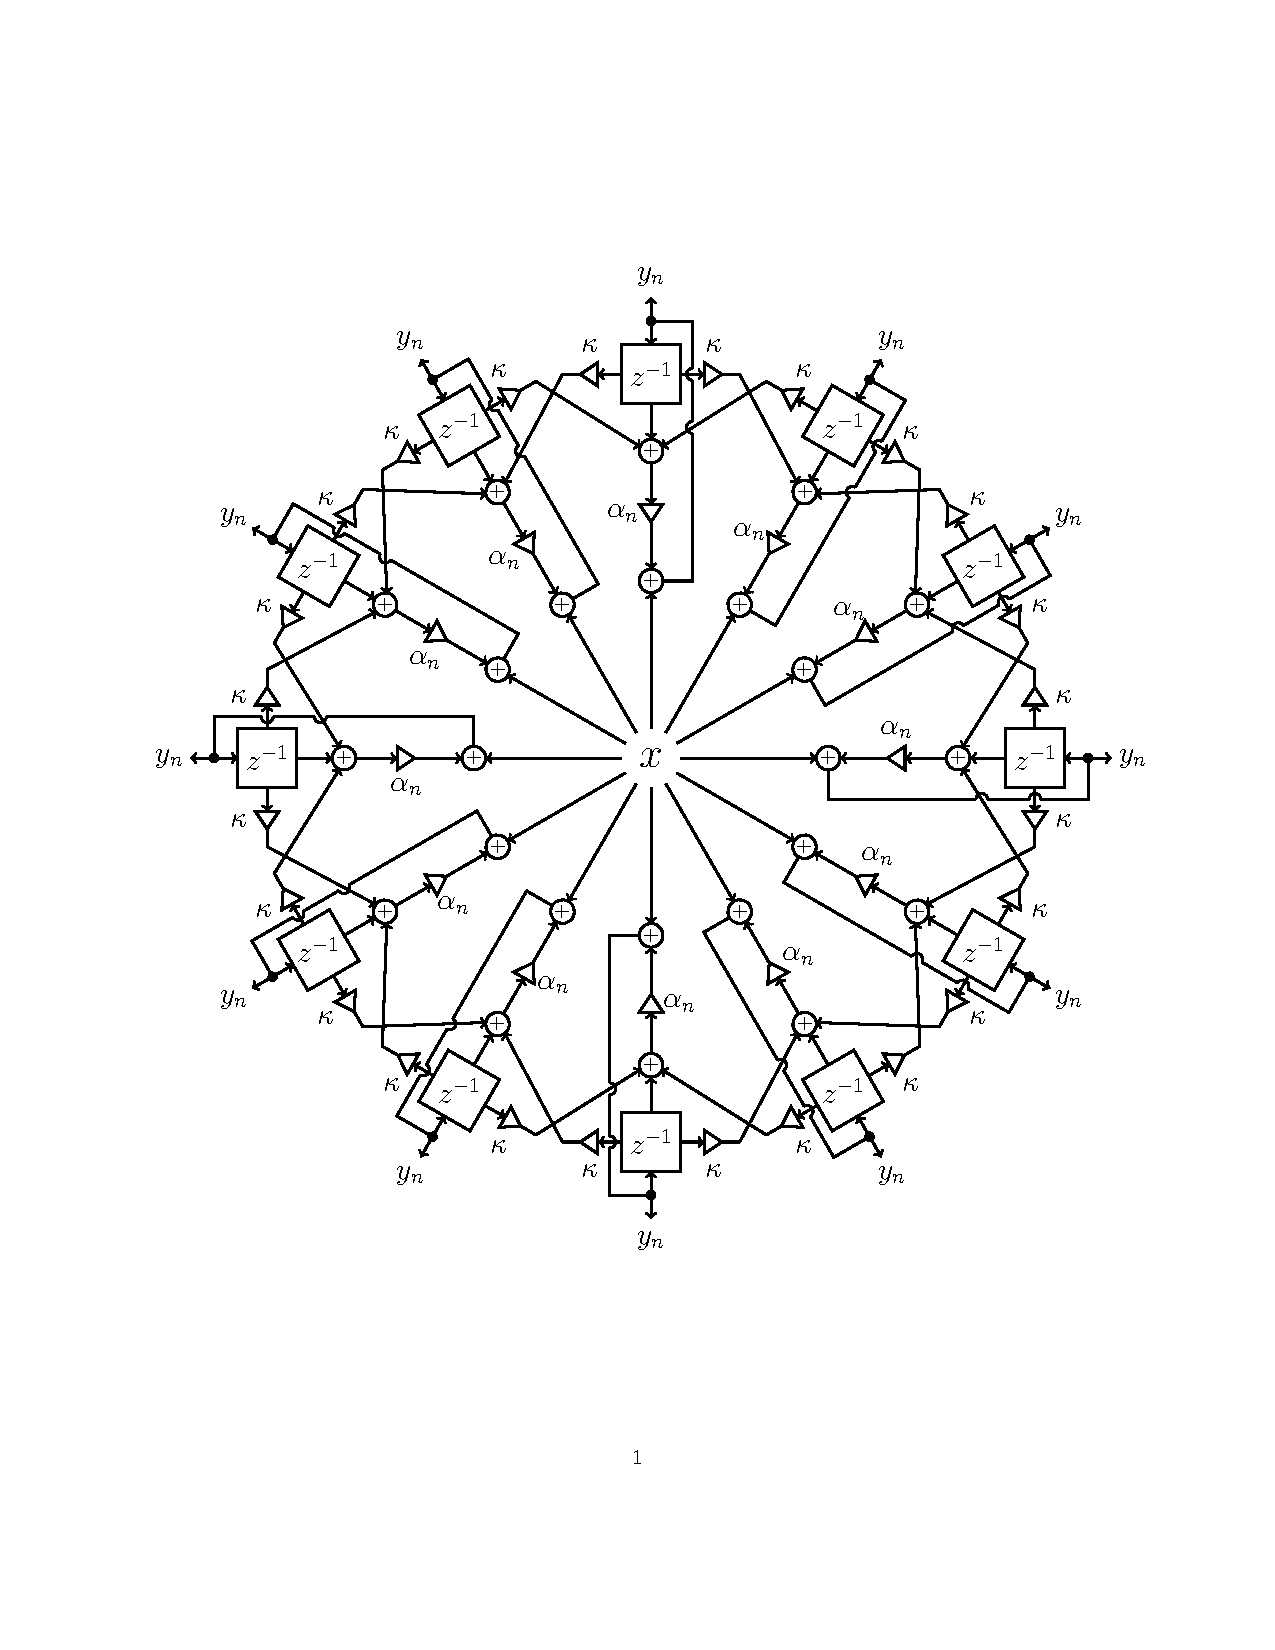
\includegraphics[width=10cm]{gabor_bank_2.pdf}
\end{figure}






\end{document}






